\documentclass[12pt, letterpaper]{article}
\usepackage[margin=1in]{geometry}
\usepackage[T1]{fontenc}
\usepackage{lmodern}
\usepackage{cmap}
\usepackage[utf8]{inputenc}
\usepackage{amsmath, amssymb, amsthm}
\usepackage{mathtools}
\usepackage{enumitem}
\usepackage{booktabs}
\usepackage{xcolor}
\usepackage{titlesec}
\usepackage{parskip}
\usepackage{hyperref}
\usepackage{fancyhdr}
\usepackage{tcolorbox}
\usepackage{graphicx}
\usepackage{caption}
\tcbuselibrary{skins, breakable}

\definecolor{darkblue}{RGB}{15,55,115}
\definecolor{midblue}{RGB}{30,100,180}
\definecolor{theorybg}{RGB}{245,250,255}
\definecolor{questionbg}{RGB}{255,252,240}
\definecolor{evencolor}{RGB}{60,0,100}

\hypersetup{colorlinks=true,linkcolor=darkblue,urlcolor=midblue,
  pdftitle={Kurlat --- A Course in Modern Macroeconomics --- Complete Solutions, Chapter 5}}

\setlength{\headheight}{14pt}
\pagestyle{fancy}
\fancyhf{}
\renewcommand{\headrulewidth}{0.4pt}
\fancyhead[L]{\small\textcolor{darkblue}{\textit{Kurlat --- A Course in Modern Macroeconomics}}}
\fancyhead[R]{\small\textcolor{darkblue}{\thepage}}
\fancyfoot[C]{\small\textcolor{gray}{Complete Solutions --- Chapter 5}}

\titleformat{\section}[block]
  {\large\bfseries\color{darkblue}}{}{0pt}{}
  [\vspace{2pt}\color{darkblue}\rule{\textwidth}{1.5pt}\vspace{4pt}]

\titleformat{\subsection}[block]
  {\normalsize\bfseries\color{midblue}}{}{0pt}{}
  [\vspace{1pt}\color{midblue}\rule{0.5\textwidth}{0.8pt}\vspace{3pt}]

\tcbset{
  theorybox/.style={
    enhanced,breakable,colback=theorybg,colframe=darkblue,
    fonttitle=\bfseries\small\color{darkblue},boxrule=0.5pt,arc=3pt,
    left=6pt,right=6pt,top=4pt,bottom=4pt,title={Key Theory},
  },
  questionbox/.style={
    enhanced,breakable,colback=questionbg,colframe=gray!60,
    fonttitle=\bfseries\small\color{gray!60!black},boxrule=0.4pt,arc=2pt,
    left=6pt,right=6pt,top=4pt,bottom=4pt,title={\textit{Question}},
  },
  oddbox/.style={
    enhanced,breakable,colback=white,colframe=darkblue,
    attach boxed title to top left={yshift=-2mm,xshift=6mm},
    boxed title style={colback=darkblue,colframe=darkblue,arc=2pt,
      boxrule=0pt,left=6pt,right=6pt,top=3pt,bottom=3pt},
    fonttitle=\bfseries\large\color{white},
    boxrule=0.8pt,arc=3pt,
    left=8pt,right=8pt,top=10pt,bottom=6pt,
  },
  evenbox/.style={
    enhanced,breakable,colback=white,colframe=evencolor,
    attach boxed title to top left={yshift=-2mm,xshift=6mm},
    boxed title style={colback=evencolor,colframe=evencolor,arc=2pt,
      boxrule=0pt,left=6pt,right=6pt,top=3pt,bottom=3pt},
    fonttitle=\bfseries\large\color{white},
    boxrule=0.8pt,arc=3pt,
    left=8pt,right=8pt,top=10pt,bottom=6pt,
  },
  databox/.style={
    enhanced,breakable,colback=gray!8,colframe=gray!55,
    fonttitle=\bfseries\small\color{gray!60!black},boxrule=0.4pt,arc=2pt,
    left=6pt,right=6pt,top=4pt,bottom=4pt,title={Numerical exercise --- see the companion code},
  },
  trapbox/.style={
    enhanced,breakable,colback=red!4,colframe=red!45!black,
    fonttitle=\bfseries\small\color{white},boxrule=0.4pt,arc=2pt,
    coltitle=white,
    left=6pt,right=6pt,top=4pt,bottom=4pt,title={Where this goes wrong},
  },
}

\newcommand{\pd}[2]{\dfrac{\partial #1}{\partial #2}}
\newcommand{\dd}[2]{\dfrac{d #1}{d #2}}
\newcommand{\MRS}{\mathrm{MRS}}
\newcommand{\MRT}{\mathrm{MRT}}
\newcommand{\MU}{\mathrm{MU}}
\newcommand{\Var}{\mathrm{Var}}
\newcommand{\Cov}{\mathrm{Cov}}
\newcommand{\E}{\mathrm{E}}
\newcommand{\MPK}{\mathrm{MPK}}
\newcommand{\MPL}{\mathrm{MPL}}
\newcommand{\stst}{^{\ast}}
\newcommand{\EST}{^{\mathrm{EST}}}
\newcommand{\TRUE}{^{\mathrm{TRUE}}}

\setlist[enumerate,1]{label=(\alph*),itemsep=6pt,parsep=2pt}
\setlist[enumerate,2]{label=(\roman*),itemsep=3pt}

\begin{document}

%======================================================================
% TITLE PAGE
%======================================================================
\begin{titlepage}
\centering
\vspace*{2.5cm}
{\Huge\bfseries\color{darkblue} A Course in Modern Macroeconomics\par}
\vspace{6pt}
{\large Pablo Kurlat (2020)\par}
\vspace{1.4cm}
{\LARGE\bfseries Complete Solutions\par}
\vspace{6pt}
{\LARGE\bfseries Chapter 5 --- Theory and Evidence\par}
\vspace{1.2cm}
{\large All nine end-of-chapter problems, 5.1--5.9 (pp.~93--99)\par}
\vspace{2cm}

\begin{tcolorbox}[theorybox,title={What is in this file},width=0.86\textwidth]
\small
Every problem carries the full question text, a step-by-step solution with no skipped
algebra, an economic reading of the result, and a verification. Numerical answers are
reproduced by the companion scripts in \texttt{Resolucao/kurlat\_ch05\_codigo/}, which
check each analytical formula against an independent computation and abort on any
mismatch.

\smallskip
Problems are grouped by \textbf{topic}, not by number, following the order of the
chapter's own sections. Blue boxes are odd-numbered problems, purple boxes even.

\smallskip
\textbf{Kurlat publishes no answer key}, so every result here is verified by other means:
executed numerical checks (marked \checkmark), internal consistency (the three GDP methods
are made to agree; steady states are substituted back), limiting cases, and cross-book
comparison with Romer (2012) ch.~1 and Jones (2020) chs.~5--6, both in \texttt{Livros/}.

\smallskip
This is a companion to \texttt{kurlat\_solutions\_ch1-4.tex} and
\texttt{kurlat\_solutions\_ch09.tex}; chapters 6--7 follow, and chapter 8 is outside the
course syllabus.
\end{tcolorbox}

\vfill
{\small MPE Insper --- Macroeconomia I --- 2026, 3\textordmasculine{} trimestre \quad$\cdot$\quad
Aula 3 --- Lista 2\par}
\end{titlepage}

\tableofcontents
\newpage

%======================================================================
\section{Chapter 5 \quad Theory and Evidence}
%======================================================================

\begin{tcolorbox}[theorybox,title={Chapter 5 Overview}]
Chapter 4 built the Solow model. Chapter 5 asks whether it survives contact with data, and
the whole chapter is organised around one move: \textbf{put numbers on the model, then see
what breaks}.

\smallskip
\textbf{The calibration (\S5.2).} $\alpha=0.35$ from the labour share; $g=0.015$ from US GDP
per capita since 1800; $n=0.01$ from US population since 1950; $\delta=0.04$; $s=0.2$ from
the investment rate. These five numbers are used again and again below, and they are
mutually consistent: they imply
\[
\frac{K}{Y}=\frac{s}{\delta+n+g}=3.08,
\qquad
r=\alpha\,\frac{\delta+n+g}{s}-\delta=7.4\%,
\]
the first of which matches the data and the second of which does not (observed safe real
rates are 1--2\%). Holding both facts in view is the point of the section.

\smallskip
\textbf{The capital-accumulation hypothesis (\S5.3).} If countries differed only in $K/L$,
poor countries would grow faster. Differentiating the transition gives
\[
g_y \;=\; s\,f'(k_t)-\alpha\delta,
\tag{5.3.1}
\]
which is decreasing in $k_t$: \emph{convergence}. The data (Fig.~3.3.1) show no such
pattern, so the conjecture fails and something other than capital must differ.

\smallskip
\textbf{Growth accounting (\S5.4).} A first-order Taylor expansion of $Y=F(K,L,A)$ gives
\[
g_Y=\underbrace{\alpha}_{\text{capital share}}g_K
   +\underbrace{(1-\alpha)}_{\text{labour share}}g_L
   +\underbrace{\text{Solow residual}}_{\text{TFP}} .
\tag{5.4.2}
\]
The key insight is that \emph{factor shares are the right weights}, because in a competitive
economy each share equals the corresponding output elasticity. Everything on the right is
measurable except the last term, which is therefore obtained as a residual.

\smallskip
\textbf{Where TFP differences come from (\S5.5).} Human capital, institutions and
misallocation (Hsieh and Klenow, 2009). The exercises hammer one particular channel:
\emph{a measurement error in an input shows up as a difference in measured TFP}. Problems
5.4, 5.5 and 5.9 are three versions of the same trap, and they are the reason a residual
should never be read as ``technology'' without argument.
\end{tcolorbox}

%---- Topic: Calibration and the Speed of Convergence ----
\subsection{Calibration and the Speed of Convergence}

%------- 5.1 -------
% Topic: Calibration and the Speed of Convergence
% Keywords: calibration, law of motion (4.5.3), steady state, transition, population growth
\begin{tcolorbox}[oddbox,title={Problem 5.1 \quad Quantifying the Solow Model}]
\begin{tcolorbox}[questionbox]
Suppose the economy is described by the Solow growth model with the parameter values we used
in Section 5.2.\\[3pt]
(a) Suppose the economy starts out with a level of GDP per efficiency unit of labor that is
only 10\% of its steady state level, i.e.\ $\tilde y_0=0.1\,\tilde y_{ss}$. What is the
initial capital stock $\tilde k_0$? Use a spreadsheet to compute $\tilde k_t$ and
$\tilde y_t$ for $t=1,2,\dots,100$. How many years does it take for
$\tilde y_t/\tilde y_{ss}>0.95$?\\[3pt]
(b) Suppose the economy begins in steady state but there is a fall in the rate of population
growth from $n=0.01$ to $n=0$. How much higher will GDP per efficiency unit of labor be in
the new steady state? Use a spreadsheet to compute $\tilde k_t$ and $\tilde y_t$ for
$t=1,2,\dots,100$. How many years does it take for $\tilde y_t/\tilde y_{ss}>0.95$?
\end{tcolorbox}

\textbf{Setup.} The calibration of \S5.2 is
\[
\alpha=0.35,\qquad s=0.20,\qquad \delta=0.04,\qquad n=0.01,\qquad g=0.015,
\]
with $\tilde y=f(\tilde k)=\tilde k^{\alpha}$ and the law of motion (4.5.3)
\[
\tilde k_{t+1}=\tilde k_t+\frac{s\,\tilde k_t^{\alpha}-(\delta+n+g)\,\tilde k_t}{1+n+g}.
\tag{$\ast$}
\]
Setting $\Delta\tilde k=0$ gives the steady state
\[
\tilde k\stst=\left(\frac{s}{\delta+n+g}\right)^{\frac{1}{1-\alpha}},
\qquad
\tilde y\stst=\left(\frac{s}{\delta+n+g}\right)^{\frac{\alpha}{1-\alpha}} .
\]
With $\delta+n+g=0.065$ and $s/(\delta+n+g)=3.0769$,
\[
\tilde k\stst=3.0769^{1/0.65}=\boxed{5.6357},
\qquad
\tilde y\stst=3.0769^{0.35/0.65}=\boxed{1.8316},
\]
and $\tilde k\stst/\tilde y\stst=3.0769=s/(\delta+n+g)$, which is exactly (5.2.1).
\checkmark

\textbf{Solution:}
\begin{enumerate}

\item \textbf{Starting 90\% below.} Output, not capital, is at 10\% of its steady-state
value, so invert the production function:
\[
\tilde y_0=0.1\,\tilde y\stst
\;\Longleftrightarrow\;
\tilde k_0^{\alpha}=0.1\,(\tilde k\stst)^{\alpha}
\;\Longleftrightarrow\;
\tilde k_0=0.1^{1/\alpha}\,\tilde k\stst .
\]
With $\alpha=0.35$, $0.1^{1/0.35}=0.1^{2.857}=1.3895\times10^{-3}$, so
\[
\boxed{\tilde k_0=1.3895\times10^{-3}\times 5.6357=0.007831},
\]
which is only $0.139\%$ of $\tilde k\stst$.

\smallskip
\emph{This is the first thing to notice, and it is not a rounding artefact.} Because
$\alpha$ is small, output is very insensitive to capital: to lose 90\% of output you must
lose 99.86\% of the capital stock. Countries that are ten times poorer than the US are
nowhere near $1/700$ of its capital per worker, which is the same arithmetic that kills the
capital-accumulation hypothesis in \S5.3.

\smallskip
Iterating ($\ast$) from $\tilde k_0$:
\begin{center}
\begin{tabular}{@{}rrr@{}}
\toprule
$t$ & $\tilde k_t$ & $\tilde y_t/\tilde y\stst$ \\
\midrule
0   & 0.0078 & 0.1000 \\
10  & 1.0148 & 0.5488 \\
25  & 2.8355 & 0.7863 \\
50  & 4.5796 & 0.9299 \\
\textbf{58}  & \textbf{4.8733} & \textbf{0.9504} \\
75  & 5.2579 & 0.9760 \\
100 & 5.5027 & 0.9917 \\
\bottomrule
\end{tabular}
\end{center}
The ratio first exceeds $0.95$ at
\[
\boxed{t=58\ \text{years}} .
\]
\checkmark\ (computed in \texttt{ch05\_numerico.py}, and unchanged if one uses the exact law
of motion instead of ($\ast$) --- see the trap box below).

\item \textbf{A fall in population growth.} Only $\delta+n+g$ changes, from $0.065$ to
$0.055$. Since $\tilde y\stst\propto(s/(\delta+n+g))^{\alpha/(1-\alpha)}$,
\[
\frac{\tilde y\stst_{\text{new}}}{\tilde y\stst_{\text{old}}}
=\left(\frac{\delta+n_{\text{old}}+g}{\delta+n_{\text{new}}+g}\right)^{\frac{\alpha}{1-\alpha}}
=\left(\frac{0.065}{0.055}\right)^{0.5385}
=1.0941 ,
\]
so GDP per efficiency unit of labour is
\[
\boxed{9.41\%\ \text{higher}}
\]
in the new steady state, with $\tilde k\stst$ rising from $5.6357$ to $7.2873$ and
$\tilde y\stst$ from $1.8316$ to $2.0040$. \checkmark

\smallskip
Iterating ($\ast$) with $n=0$ from $\tilde k_0=5.6357$:
\begin{center}
\begin{tabular}{@{}rrr@{}}
\toprule
$t$ & $\tilde k_t$ & $\tilde y_t/\tilde y\stst_{\text{new}}$ \\
\midrule
0   & 5.6357 & 0.9140 \\
5   & 5.8961 & 0.9285 \\
10  & 6.1171 & 0.9406 \\
\textbf{15}  & \textbf{6.3040} & \textbf{0.9505} \\
20  & 6.4618 & 0.9588 \\
40  & 6.8798 & 0.9801 \\
100 & 7.2394 & 0.9977 \\
\bottomrule
\end{tabular}
\end{center}
The ratio exceeds $0.95$ at
\[
\boxed{t=15\ \text{years}} .
\]
\checkmark

\end{enumerate}

\smallskip
\emph{Reading.} The two parts look like the same experiment run twice, and the contrast
between $58$ years and $15$ years is the lesson. Convergence in the Solow model happens at a
roughly constant \emph{proportional} rate --- Problem 5.2 shows it is
$(1-\alpha)(\delta+n+g)\approx 3.6\%$ per year here --- so the time it takes is governed
almost entirely by \emph{how far the economy starts from its target}, not by what moved it.
Part (a) starts at 10\% of the target and needs six decades; part (b) starts at 91\% of the
target and needs fifteen years.

\smallskip
Two further points on part (b) that are easy to miss:
\begin{itemize}[leftmargin=1.3em,itemsep=2pt,topsep=3pt]
\item Slower population growth raises the \emph{level} of GDP per person by $9.41\%$ but
      leaves its long-run \emph{growth rate} at $g=1.5\%$. Level effects and growth effects
      are different objects, and only technological progress does the second.
\item Total GDP grows more slowly afterwards, at $g$ instead of $n+g$. A country that likes
      the level effect must accept the aggregate one; which of the two matters depends on
      whether the question is about living standards or about the size of the economy.
\end{itemize}

\begin{tcolorbox}[trapbox]
Kurlat's (4.5.3) drops the $ng$ cross-term, so ($\ast$) is an approximation to the exact
recursion
\[
\tilde k_{t+1}=\frac{(1-\delta)\tilde k_t+s\,\tilde k_t^{\alpha}}{(1+n)(1+g)} .
\]
It is worth checking that the answers do not depend on which one you use. With the exact
version, $\tilde k\stst=5.6158$ instead of $5.6357$, the steady-state gain in part (b) is
$9.55\%$ instead of $9.41\%$, and the two answers become $58$ years and $16$ years. The
qualitative conclusion is identical and the quantitative one moves by at most one year;
\texttt{problema\_5\_1\_exato()} runs this check.

\smallskip
The genuine error to avoid is setting $\tilde k_0=0.1\,\tilde k\stst$. That is a 90\% cut in
\emph{capital}, which leaves output at $0.1^{0.35}=45\%$ of steady state, not 10\%, and the
answer to (a) then comes out around 34 years.
\end{tcolorbox}

\begin{center}
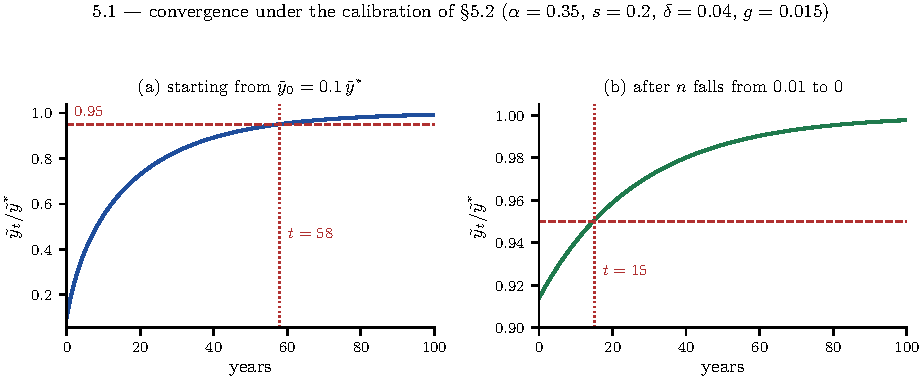
\includegraphics[width=\linewidth]{fig/fig_k5_1_convergencia.pdf}\\[3pt]
\captionof{figure}{Problem 5.1. Left: the transition from $\tilde y_0=0.1\tilde y\stst$.
Right: the transition after $n$ falls to zero. Same model, same speed --- different starting
distance.}
\label{fig:conv51}
\end{center}
\end{tcolorbox}

%------- 5.2 -------
% Topic: Calibration and the Speed of Convergence
% Keywords: convergence, equation (5.3.1), half-life, first-order approximation, beta-convergence
\begin{tcolorbox}[evenbox,title={Problem 5.2 \quad The Speed of Convergence}]
\begin{tcolorbox}[questionbox]
Suppose the economy is described by the Solow growth model with a Cobb-Douglas production
function, no population growth and no technological progress. The economy is not in steady
state. GDP per capita in period $t$ is $y_t=\phi\,y_{ss}$, with $\phi\in(0,1)$.\\[3pt]
(a) How far away from steady state is the capital stock? Find an expression for the level of
$k_t/k_{ss}$ that would be consistent with $y_t=\phi y_{ss}$, in terms of $\phi$ and
parameters.\\[3pt]
(b) Find an expression for $k_{ss}$, the steady state level of capital, in terms of
parameters.\\[3pt]
(c) Use your results from parts (a) and (b) and equation (5.3.1) to find an expression for
$g_y$, the rate of growth of GDP, as a function of $\phi$ and parameters.\\[3pt]
(d) Let $\alpha=0.35$ and $\delta=0.04$. Compute $g_y$ for an economy whose GDP is
$\phi=0.8$ times its steady-state level. Compute $g_y/(1-\phi)$. What fraction of the gap
between $y_t$ and $y_{ss}$ does the economy close in one year? Repeat this calculation for
$\phi=0.9$ and $\phi=0.99$.
\end{tcolorbox}

\textbf{Solution:}
\begin{enumerate}

\item Output is $y=k^{\alpha}$, so
\[
\phi=\frac{y_t}{y_{ss}}=\left(\frac{k_t}{k_{ss}}\right)^{\alpha}
\qquad\Longrightarrow\qquad
\boxed{\frac{k_t}{k_{ss}}=\phi^{1/\alpha}} .
\]
Since $1/\alpha=2.86>1$ and $\phi<1$, capital is proportionally \emph{much} further from its
steady state than output is: at $\phi=0.8$, $k_t/k_{ss}=0.8^{2.857}=0.53$.

\item With $n=g=0$ the law of motion is $\Delta k=s k^{\alpha}-\delta k$, so
$s k_{ss}^{\alpha}=\delta k_{ss}$ and
\[
\boxed{k_{ss}=\left(\frac{s}{\delta}\right)^{\frac{1}{1-\alpha}}} ,
\qquad\text{equivalently}\qquad
\frac{k_{ss}^{\alpha-1}}{1}=\frac{\delta}{s}.
\tag{5.2.b}
\]
The second form is the one that will be used --- it says $s\,k_{ss}^{\alpha-1}=\delta$.

\item Equation (5.3.1) for a Cobb-Douglas $f(k)=k^{\alpha}$ reads
\[
g_y = s f'(k_t)-\alpha\delta = s\,\alpha\,k_t^{\alpha-1}-\alpha\delta .
\]
Substitute $k_t=\phi^{1/\alpha}k_{ss}$:
\[
k_t^{\alpha-1}=\phi^{\frac{\alpha-1}{\alpha}}\,k_{ss}^{\alpha-1}
=\phi^{-\frac{1-\alpha}{\alpha}}\cdot\frac{\delta}{s},
\]
where the last step uses (5.2.b). Therefore
\[
g_y=s\alpha\cdot\phi^{-\frac{1-\alpha}{\alpha}}\frac{\delta}{s}-\alpha\delta
\qquad\Longrightarrow\qquad
\boxed{\;g_y(\phi)=\alpha\delta\left(\phi^{-\frac{1-\alpha}{\alpha}}-1\right)\;}
\]
Note that $s$ has cancelled: given how far output is from \emph{its own} steady state, the
growth rate does not depend on the saving rate. Two checks: $g_y(1)=0$ \checkmark, and
$g_y$ is decreasing in $\phi$ \checkmark, which is convergence.

\item With $\alpha\delta=0.014$ and $(1-\alpha)/\alpha=1.8571$:

\begin{center}
\begin{tabular}{@{}rrrrr@{}}
\toprule
$\phi$ & $\phi^{-1.8571}$ & $g_y$ & $g_y/(1-\phi)$ & $g_y\phi/(1-\phi)$ \\
       &                  &       & (as asked)     & (gap actually closed) \\
\midrule
0.80 & 1.5134 & 0.7189\% & 3.5943\% & 2.8755\% \\
0.90 & 1.2161 & 0.3026\% & 3.0257\% & 2.7232\% \\
0.99 & 1.0188 & 0.0264\% & 2.6376\% & 2.6113\% \\
\bottomrule
\end{tabular}
\end{center}
\checkmark\ Each row is confirmed in \texttt{ch05\_numerico.py} against one exact iteration of
$k_{t+1}=k_t+sk_t^{\alpha}-\delta k_t$, which reproduces $g_y$ to within $0.7\%$ of its own
value --- the small discrepancy is the first-order approximation inside (5.3.1), not an
algebra error.

\smallskip
\emph{Which column answers ``what fraction of the gap is closed''?} The gap is
$y_{ss}-y_t=(1-\phi)y_{ss}$, and one year of growth adds $g_y\,y_t=g_y\phi\,y_{ss}$, so the
fraction closed is $g_y\phi/(1-\phi)$ --- the last column. The exercise asks for
$g_y/(1-\phi)$, which is the same object divided by $\phi$ and therefore slightly larger;
the two agree to three digits once $\phi$ is near one, which is the case the exercise is
really about.

\end{enumerate}

\smallskip
\emph{Reading, and this is the number to remember.} Take $\phi\to1$ and expand
$\phi^{-(1-\alpha)/\alpha}\approx 1+\frac{1-\alpha}{\alpha}(1-\phi)$:
\[
g_y \;\approx\; \alpha\delta\cdot\frac{1-\alpha}{\alpha}(1-\phi)
\;=\;\underbrace{\delta(1-\alpha)}_{\lambda}\,(1-\phi).
\]
So the economy closes a constant fraction
\[
\lambda=\delta(1-\alpha)=0.04\times0.65=\boxed{2.6\%}
\]
of its remaining gap every year, and the table converges to exactly that: $3.59\%$,
$3.03\%$, $2.64\%$. In the general case with population growth and technological progress
the same derivation gives $\lambda=(1-\alpha)(\delta+n+g)$, which under the \S5.2
calibration is $0.65\times0.065=4.2\%$.

\smallskip
The implied \textbf{half-life} is $\ln 2/\lambda=0.693/0.026\approx 27$ years here (about 16
years under the full calibration). This is the single most-quoted quantitative prediction of
the Solow model, and it is the number that empirical growth regressions --- the
``2\% convergence'' literature --- were built to test. That the model delivers roughly the
right speed while failing the level test of \S5.3 is the tension the chapter is about.

\begin{center}
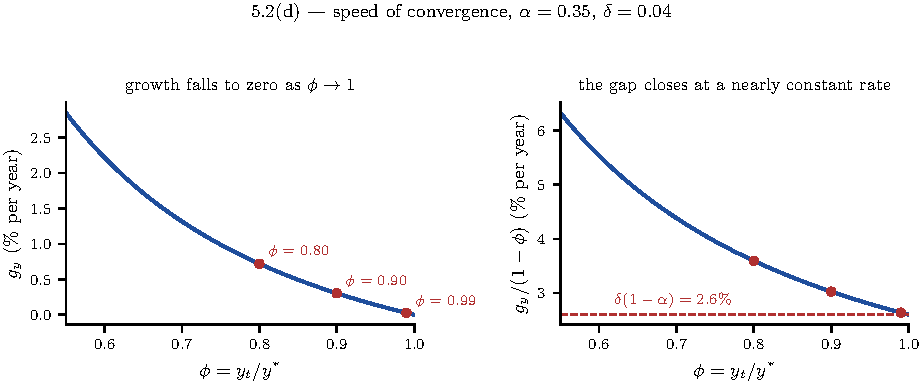
\includegraphics[width=\linewidth]{fig/fig_k5_2_velocidade.pdf}\\[3pt]
\captionof{figure}{Problem 5.2(d). Left: growth vanishes as the economy approaches its
steady state. Right: the \emph{proportional} speed at which the gap closes is nearly
constant, and tends to $\delta(1-\alpha)$.}
\label{fig:vel52}
\end{center}
\end{tcolorbox}

%---- Topic: Growth Accounting and the Sources of Growth ----
\subsection{Growth Accounting and the Sources of Growth}

%------- 5.3 -------
% Topic: Growth Accounting and the Sources of Growth
% Keywords: Solow residual, proximate vs ultimate cause, balanced growth, equation (5.4.2)
\begin{tcolorbox}[oddbox,title={Problem 5.3 \quad Causes of Growth and Growth Accounting}]
\begin{tcolorbox}[questionbox]
Suppose an economy is well described by the steady state of the Solow Growth Model with
constant technological progress and no population growth. Imagine we take data from this
economy and do a growth-accounting exercise. How much growth will we attribute to capital
accumulation and how much to technology? How does this relate to the result that says that
without technological progress there would be no growth in the steady state?
\end{tcolorbox}

\textbf{Solution.} Write the production function in the labour-augmenting form
$Y_t=K_t^{\alpha}(A_tL_t)^{1-\alpha}$ with $g_A=g$, $g_L=0$.

\smallskip
\textbf{Step 1: what the variables actually do in this steady state.} By definition of a
steady state, $\tilde k=K/(AL)$ is constant, so $K$ grows at the same rate as $AL$:
\[
g_K=g_A+g_L=g .
\]
And $Y=\tilde k^{\alpha}AL$ with $\tilde k$ constant gives $g_Y=g$ as well. Everything grows
at $g$; this is the balanced growth path.

\smallskip
\textbf{Step 2: run (5.4.2).} The capital share is $\alpha$, the labour share $1-\alpha$:
\[
\underbrace{g_Y}_{g}
=\underbrace{\alpha\,g_K}_{\alpha g}
+\underbrace{(1-\alpha)g_L}_{0}
+\underbrace{\text{residual}}_{?}
\qquad\Longrightarrow\qquad
\text{residual}=g-\alpha g=(1-\alpha)g .
\]
So the exercise attributes
\[
\boxed{\text{a fraction }\alpha=35\%\text{ of growth to capital accumulation}}
\]
\[
\boxed{\text{and a fraction }1-\alpha=65\%\text{ to technology.}}
\]
Under the \S5.2 calibration, of the $1.5\%$ annual growth, $0.53$ points are labelled
``capital'' and $0.97$ points are the Solow residual. \checkmark

\smallskip
\emph{Consistency check.} Rewrite the production function in Hicks-neutral form,
$Y=\tilde A K^{\alpha}L^{1-\alpha}$ with $\tilde A\equiv A^{1-\alpha}$. Then
$g_{\tilde A}=(1-\alpha)g$, which is exactly the residual. The two ways of writing
technology give the same accounting, as they must. \checkmark

\smallskip
\textbf{How this relates to ``no technological progress, no growth''.} It looks like a
contradiction: Proposition 4.3 says technology is the \emph{only} source of long-run growth,
yet the accounting gives it only 65\% of the credit. Both statements are true, because they
answer different questions.

\begin{itemize}[leftmargin=1.3em,itemsep=3pt,topsep=3pt]
\item Growth accounting is a \textbf{proximate} decomposition. It asks: holding the other
      inputs fixed, how much of the observed change in output does each observed change in
      an input mechanically explain? It treats $g_K$ as a fact about the world, with no view
      on where it came from.
\item The Solow model gives the \textbf{ultimate} cause. Here capital grows \emph{only
      because} technology grows: $g_K=g$ is not an independent parameter, it is an
      equilibrium response. Set $g=0$ and the whole thing collapses --- $g_K=0$ and
      $g_Y=0$. Every one of the $0.53$ points labelled ``capital'' would disappear.
\end{itemize}

\smallskip
Formally, the total derivative of steady-state growth with respect to $g$ is
\[
\frac{dg_Y}{dg}
=\underbrace{\alpha\frac{dg_K}{dg}}_{\alpha\cdot 1}+\underbrace{(1-\alpha)}_{\text{direct}}
=1,
\]
against a partial derivative, holding $g_K$ fixed, of only $1-\alpha$. Growth accounting
reports the partial; the model reports the total.

\smallskip
\emph{Reading.} This is the standard caution about the Solow residual, and it runs in both
directions. Growth accounting \emph{understates} the role of anything that induces capital
accumulation --- technology here, but equally an institutional reform or a fall in the cost
of investment goods. It \emph{overstates} the role of capital in exactly the same amount.
A decomposition that gives capital 35\% of Soviet growth (Example 5.1) is not a claim that
capital was 35\% of the reason; it is a claim about the arithmetic of a Taylor expansion.
One can convert a proximate share into an ultimate one by dividing the residual by
$1-\alpha$: here $(1-\alpha)g/(1-\alpha)=g$, technology gets 100\%, which is Proposition 4.3
recovered.
\end{tcolorbox}

%------- 5.6 -------
% Topic: Growth Accounting and the Sources of Growth
% Keywords: interest rate, marginal product of capital, transition dynamics, identification
\begin{tcolorbox}[evenbox,title={Problem 5.6 \quad Interest Rates}]
\begin{tcolorbox}[questionbox]
Suppose we observe that Usuria (a closed economy) grows at approximately 6\% a year, and we
are trying to understand why. We know the labor force has been constant.\\[3pt]
$\bullet$ \textbf{Conjecture 1:} The economy has been at a steady-state-with-technological-progress.
There has been capital accumulation just to maintain $K/(AL)$ constant but the cause of
growth has been TFP growth.\\[3pt]
$\bullet$ \textbf{Conjecture 2:} The economy started from a very low level of capital stock (below
steady state) and has been growing because it is converging to the steady state, but TFP has
been constant.\\[3pt]
Ideally, if we wanted to distinguish between Conjecture 1 and Conjecture 2 we could do a
growth-accounting exercise. Unfortunately, Usuria does not collect reliable statistics on
capital accumulation that would enable us to do this. We do, however, have data on interest
rates in Usuria. How would one use these data to distinguish between Conjecture 1 and
Conjecture 2? Be as mathematically precise as possible.
\end{tcolorbox}

\textbf{The idea in one line.} The interest rate \emph{is} a measurement of the capital
stock. We cannot see $K$, but $r$ is a monotone function of $K/Y$, so the behaviour of $r$
tells us what $K$ is doing.

\smallskip
\textbf{Step 1: the link.} With $Y=K^{\alpha}(AL)^{1-\alpha}$ and competitive factor
markets,
\[
r_t=F_K(K_t,A_tL_t)-\delta=\alpha K_t^{\alpha-1}(A_tL_t)^{1-\alpha}-\delta
=\alpha\,\frac{Y_t}{K_t}-\delta ,
\qquad\text{i.e.}\qquad
\frac{K_t}{Y_t}=\frac{\alpha}{r_t+\delta}.
\tag{5.6.1}
\]
This holds on \emph{any} path, in or out of steady state, and requires no data on $K$
itself.

\smallskip
\textbf{Step 2: what each conjecture implies.} Take logs of (5.6.1) and differentiate:
\[
\frac{d\ln(r_t+\delta)}{dt}=g_Y-g_K .
\tag{5.6.2}
\]

\begin{itemize}[leftmargin=1.3em,itemsep=4pt,topsep=3pt]
\item \textbf{Conjecture 1.} On a balanced growth path $K/(AL)$ is constant and $L$ is
      constant, so $g_K=g_A=g_Y=6\%$. Then (5.6.2) gives
      \[
      \frac{d\ln(r+\delta)}{dt}=0
      \qquad\Longrightarrow\qquad
      \boxed{r_t\ \text{is constant}} .
      \]

\item \textbf{Conjecture 2.} $A$ is constant and $L$ is constant, so all of the growth in
      $Y$ must come from $K$. Growth accounting with a zero residual gives
      \[
      g_Y=\alpha g_K
      \qquad\Longrightarrow\qquad
      g_K=\frac{g_Y}{\alpha}=\frac{0.06}{0.35}=17.1\%\ \text{per year},
      \]
      and (5.6.2) becomes
      \[
      \frac{d\ln(r+\delta)}{dt}=g_Y\left(1-\frac{1}{\alpha}\right)
      =0.06\times(1-2.857)=\boxed{-11.1\%\ \text{per year}} .
      \]
\end{itemize}

\textbf{Step 3: the test.} Regress $\ln(r_t+\delta)$ on time.
\[
\text{slope}=0 \;\Rightarrow\; \text{Conjecture 1};
\qquad
\text{slope}=g_Y\!\left(1-\tfrac{1}{\alpha}\right)<0 \;\Rightarrow\; \text{Conjecture 2}.
\]
The two predictions are not merely different in sign, they are far apart in magnitude: under
Conjecture 2 the gross return $r+\delta$ falls by a factor $e^{-1.11}=0.33$ over a single
decade. Ten years of interest-rate data settle the question, and the only auxiliary
parameters needed are $\alpha$ (readable off the labour share, which Usuria does report as
part of its GDP accounts) and $\delta$, which enters only through the level shift
$r+\delta$.

\smallskip
\textbf{A sharper version using levels.} If we are also willing to use the investment rate
$s$, the two conjectures predict very different interest rates \emph{today}. From
$g_K=sY/K-\delta$ and (5.6.1),
\[
r=\alpha\,\frac{g_K+\delta}{s}-\delta .
\]
Taking the \S5.2 values $s=0.2$, $\delta=0.04$, $\alpha=0.35$:
\begin{center}
\begin{tabular}{@{}lcc@{}}
\toprule
 & $g_K$ & implied $r$ \\
\midrule
Conjecture 1 (balanced growth, $g_K=g_Y$)   & $6.0\%$  & $13.5\%$ \\
Conjecture 2 (transition, $g_K=g_Y/\alpha$) & $17.1\%$ & $33.0\%$ \\
\bottomrule
\end{tabular}
\end{center}
\checkmark\ A 33\% real interest rate is not something one would fail to notice. The
corresponding $K/Y$ ratios are $2.6$ and $0.95$: under Conjecture 2 the economy would have
less than one year of GDP in capital, against a US figure of about three.

\smallskip
\emph{Reading.} This exercise is a small lesson in identification. Two stories generate the
same observable --- 6\% growth --- and are distinguished by a \emph{different} observable
that the theory ties to the unobserved variable. It is also a reality check on Conjecture 2
generally: a 17\% annual capital growth rate sustained for years is enormous, and the
implied interest rate is far above anything ever measured. That is essentially the argument
Lucas (1990) makes about why capital does not flow to poor countries, and it is another way
of stating why \S5.3 rejects the capital-accumulation hypothesis.
\end{tcolorbox}

%---- Topic: National Accounts, Factor Shares and the Golden Rule ----
\subsection{National Accounts, Factor Shares and the Golden Rule}

%------- 5.7 -------
% Topic: National Accounts, Factor Shares and the Golden Rule
% Keywords: three GDP methods, imports, government at cost, factor shares, growth accounting
\begin{tcolorbox}[oddbox,title={Problem 5.7 \quad GDP Accounting, Interest Rates and Growth Accounting}]
\begin{tcolorbox}[questionbox]
Proletaria is a mythical country in Central Asia, where the currency is the ruble. The
exchange rate is 10 rubles per euro. Suppose the production function in Proletaria is given
by $Y=K^{\alpha}L^{1-\alpha}$.\\[3pt]
(a) Find expressions for the output-to-capital ratio $Y/K$ and the marginal product of
capital $F_K$ as functions of $K$ and $L$.\\[3pt]
During 2014, the following events took place in Proletaria.
\begin{itemize}[leftmargin=1.1em,itemsep=1pt,topsep=2pt]
\item Kapitas, the main manufacturer in the country, imported an industrial welder made in
Germany, for which it paid 1,000 euro.
\item By the end of the year, the industrial welder was no longer new. Its estimated value
in the resale market was 960 euro.
\item 100 workers worked for Kapitas the entire year making screws and nails, using the new
welder. Each of them received wages for 350 rubles.
\item Each of the Kapitas workers paid 100 rubles in income taxes.
\item The total output of Kapitas consisted of 1 million screws and 1 million nails. All of
it was exported to Austria for a total of 4,000 euro.
\item The government of Proletaria employed one of the 100 workers as Chief of the Secret
Police (in addition to his factory job) to maintain law and order, and paid her a salary of
10,000 rubles.
\item The workers ate beef imported from France, which cost a total of 2,500 euro.
\end{itemize}
(b) Construct GDP accounts (in rubles) for Proletaria by production, income and expenditure.\\
(c) What were the income shares of labor and capital?\\
(d) Suppose that we know that the capital stock in Proletaria is 100,000 rubles and that the
depreciation rate of the industrial welder is typical for this country's capital stock. What
interest rate should we expect to observe?\\
(e) During 2015, additional investment in Proletaria has exceeded depreciation so that the
capital stock now stands at 120,000 rubles. The labor force also grew thanks to immigration,
and now consists of 105 workers instead of 100. GDP during 2015 was 55,000 rubles (prices
were constant). How much of the growth in GDP between 2014 and 2015 can be attributed to
growth in Total Factor Productivity?
\end{tcolorbox}

\textbf{Solution:}
\begin{enumerate}

\item Divide the production function by $K$ and differentiate it:
\[
\frac{Y}{K}=K^{\alpha-1}L^{1-\alpha}=\boxed{\left(\frac{L}{K}\right)^{1-\alpha}},
\qquad
F_K=\alpha K^{\alpha-1}L^{1-\alpha}=\boxed{\alpha\left(\frac{L}{K}\right)^{1-\alpha}
=\alpha\,\frac{Y}{K}} .
\]
The second identity, $F_K=\alpha Y/K$, is the workhorse of parts (d) and (e): with
Cobb-Douglas, the marginal product of capital is the capital share times the output-capital
ratio, and both are observable.

\item Convert everything at 10 rubles per euro: the welder costs $10{,}000$ rubles and is
worth $9{,}600$ at year-end; the exports are $40{,}000$; the beef is $25{,}000$.

\smallskip
\textbf{Production (value added).}
\begin{center}
\begin{tabular}{@{}lrr@{}}
\toprule
Producer & Gross output & Value added \\
\midrule
Kapitas (screws and nails) & 40{,}000 & 40{,}000 \\
Government (police services, valued at cost) & 10{,}000 & 10{,}000 \\
\midrule
\textbf{GDP} & & \textbf{50{,}000} \\
\bottomrule
\end{tabular}
\end{center}
Kapitas uses no intermediate inputs: the welder is \emph{capital}, not an intermediate good,
so it is not netted out of value added. The beef and the welder are produced abroad and
contribute nothing to Proletarian production.

\smallskip
\textbf{Income.}
\begin{center}
\begin{tabular}{@{}lr@{}}
\toprule
Wages, Kapitas ($100\times350$) & 35{,}000 \\
Wages, government (the police chief's salary) & 10{,}000 \\
Capital income / operating surplus, Kapitas ($40{,}000-35{,}000$) & 5{,}000 \\
\midrule
\textbf{GDP} & \textbf{50{,}000} \\
\bottomrule
\end{tabular}
\end{center}

\smallskip
\textbf{Expenditure.}
\begin{center}
\begin{tabular}{@{}lr@{}}
\toprule
$C$ \ (beef) & 25{,}000 \\
$I$ \ (welder) & 10{,}000 \\
$G$ \ (police services) & 10{,}000 \\
$X$ \ (screws and nails) & 40{,}000 \\
$-M$ \ (welder $10{,}000$ + beef $25{,}000$) & $-35{,}000$ \\
\midrule
\textbf{GDP} & \textbf{50{,}000} \\
\bottomrule
\end{tabular}
\end{center}
\checkmark\ The three methods agree at $50{,}000$ rubles, which is the check the exercise is
built around.

\smallskip
\emph{Four traps in this list, and each is deliberate.}
\begin{itemize}[leftmargin=1.3em,itemsep=2pt,topsep=3pt]
\item \textbf{Income taxes ($10{,}000$ rubles) are not in GDP anywhere.} They are a transfer
      from households to the government; the production they finance is already counted at
      the salaries paid. Adding them would double-count.
\item \textbf{The police chief's services are counted at cost}, $10{,}000$ rubles, because
      they are not sold in a market. This is the convention of \S1.3 and it is why the
      largest single item of Proletarian value added is a service with no price.
\item \textbf{The police chief holds two jobs.} She is one of the 100 factory workers, so
      the labour force is 100, not 101. Her factory wage ($350$) is inside the $35{,}000$
      and her government salary ($10{,}000$) is on top of it.
\item \textbf{Depreciation ($400$ rubles) does not appear.} These are \emph{gross} accounts;
      the $400$ would be subtracted to get NDP, and it is used in part (d) to pin $\delta$.
\end{itemize}

\item Read the shares off the income account:
\[
\text{labour share}=\frac{35{,}000+10{,}000}{50{,}000}=\boxed{0.90},
\quad
\text{capital share}=\alpha=\frac{5{,}000}{50{,}000}=\boxed{0.10} .
\]
The shares sum to one, as the income method requires. \checkmark

\smallskip
A capital share of $0.10$ is very low --- the empirical benchmark is $0.35$ --- and the
reason is visible in the accounts: a fifth of Proletarian GDP is a government service valued
at the wage bill, which is by construction 100\% labour income. Toy economies with a large
imputed public sector always look labour-intensive.

\item Depreciation of the welder: it lost $10{,}000-9{,}600=400$ rubles of value on a stock
of $10{,}000$, so
\[
\delta=\frac{400}{10{,}000}=0.04 .
\]
Then, using $F_K=\alpha Y/K$ from part (a),
\[
r=F_K-\delta=\alpha\frac{Y}{K}-\delta
=0.10\times\frac{50{,}000}{100{,}000}-0.04
=0.05-0.04=\boxed{1\%} .
\]
\checkmark

\smallskip
The number is low, and part (c) explains why: with a capital share of only $0.10$, capital
earns $5{,}000$ a year on a stock of $100{,}000$, a gross return of 5\%, of which four
points are eaten by depreciation. Note also the internal consistency: $K/Y=2$ and
$\alpha/(r+\delta)=0.10/0.05=2$. \checkmark

\item Growth accounting, equation (5.4.2), with the shares from part (c):
\[
g_Y=\frac{55{,}000}{50{,}000}-1=10\%,\qquad
g_K=\frac{120{,}000}{100{,}000}-1=20\%,\qquad
g_L=\frac{105}{100}-1=5\% ,
\]
\[
\text{TFP}=g_Y-\alpha g_K-(1-\alpha)g_L
=0.10-0.10\times0.20-0.90\times0.05 ,
\]
\[
\text{TFP}=0.10-0.02-0.045=\boxed{3.5\%} .
\]
\checkmark\ So $3.5$ of the $10$ percentage points of growth --- \textbf{35\% of it} --- is
Total Factor Productivity.

\smallskip
\emph{Reading.} Note how much the answer depends on part (c). Capital grew twice as fast as
output, which sounds like the dominant force, but it is weighted by a share of only $0.10$
and contributes just $2$ points. Labour grew half as fast but carries a weight of $0.90$ and
contributes more than twice as much. This is the whole content of ``factor shares are the
right weights'': the fast-growing input is not necessarily the important one.

\end{enumerate}
\end{tcolorbox}

%------- 5.8 -------
% Topic: National Accounts, Factor Shares and the Golden Rule
% Keywords: value added, intermediate goods, saving rate, Golden Rule, dynamic efficiency
\begin{tcolorbox}[evenbox,title={Problem 5.8 \quad National Accounts and The Golden Rule}]
\begin{tcolorbox}[questionbox]
In 2018, the following events happened in Aurum, which is a closed economy that uses the
Denarius (plural: Denarii) as its currency.
\begin{itemize}[leftmargin=1.1em,itemsep=1pt,topsep=2pt]
\item Grano, Inc.\ hired Cornelia to plant and harvest 500 tons of wheat on a large plot of
land using a tractor. Both the land and the tractor are owned by Grano, Inc. It paid
Cornelia 200 Denarii for her work on the harvest. It sold the wheat to Panem, Inc.\ for
1,000 Denarii.
\item The tractor Cornelia used was new at the beginning of the year, worth 2,000 Denarii,
and was no longer new at the end of the year: by then it was worth 1,800 Denarii.
\item Panem, Inc.\ hired Gaius to grind the wheat in its mill and produce a million loaves
of bread. It paid Gaius 1,400 Denarii for his work. It sold the bread for 4,000 Denarii to
the hungry citizens, who eat it.
\item Fabrica, Inc.\ hired Livia to build a combine harvester. It paid Livia 400 Denarii for
her work. It sold the combine harvester to Grano, Inc.\ for 1,000 Denarii.
\end{itemize}
(a) Construct GDP accounts (in Denarii) for Aurum by production, income and expenditure.\\
(b) What were the income shares of labor and capital?\\
(c) What was the savings rate?\\
(d) Assume the following: the savings rate is constant; the production function has the form
$Y=AK^{\alpha}L^{1-\alpha}$ and there is no technological progress; the depreciation rate
for the tractor is typical for the capital stock as a whole; the population is constant. In
the long run, would the level of consumption be higher if the economy slightly increased its
saving rate?
\end{tcolorbox}

\textbf{Solution:}
\begin{enumerate}

\item \textbf{Production (value added).}
\begin{center}
\begin{tabular}{@{}lrrr@{}}
\toprule
Firm & Gross output & Intermediates & Value added \\
\midrule
Grano (wheat)             & 1{,}000 & 0       & 1{,}000 \\
Panem (bread)             & 4{,}000 & 1{,}000 & 3{,}000 \\
Fabrica (combine harvester)& 1{,}000 & 0       & 1{,}000 \\
\midrule
\textbf{GDP} & & & \textbf{5{,}000} \\
\bottomrule
\end{tabular}
\end{center}
The wheat is an \emph{intermediate} good: it is bought by Panem and physically transformed
within the year, so it is netted out of Panem's value added. The combine harvester is
\emph{capital}: it is bought by Grano but survives the year, so it is not netted out of
anything and stays in GDP as investment.

\smallskip
\textbf{Income.}
\begin{center}
\begin{tabular}{@{}lrrr@{}}
\toprule
 & Wages & Capital income & Total \\
\midrule
Grano   & 200   & $1{,}000-200=800$   & 1{,}000 \\
Panem   & 1{,}400 & $4{,}000-1{,}000-1{,}400=1{,}600$ & 3{,}000 \\
Fabrica & 400   & $1{,}000-400=600$   & 1{,}000 \\
\midrule
\textbf{Total} & \textbf{2{,}000} & \textbf{3{,}000} & \textbf{5{,}000} \\
\bottomrule
\end{tabular}
\end{center}
Capital income here is gross operating surplus: it is the return to the tractor, the land and
the mill, and it includes the $200$ of depreciation.

\smallskip
\textbf{Expenditure.}
\begin{center}
\begin{tabular}{@{}lr@{}}
\toprule
$C$ \ (bread, eaten by citizens) & 4{,}000 \\
$I$ \ (combine harvester) & 1{,}000 \\
$G=0$, \ $X=M=0$ (closed economy, no government) & 0 \\
\midrule
\textbf{GDP} & \textbf{5{,}000} \\
\bottomrule
\end{tabular}
\end{center}
\checkmark\ Three methods, $5{,}000$ Denarii each.

\begin{tcolorbox}[trapbox]
The wheat and the combine harvester cost the same $1{,}000$ Denarii and are treated in
opposite ways. The test is not the price and not the buyer --- both are bought by firms ---
but whether the good \emph{survives the period}. Wheat is consumed in production this year
(intermediate, netted out); a harvester is used for years (capital, counted as investment).
Netting out the harvester would give GDP $=4{,}000$; counting the wheat would give
$6{,}000$. Only $5{,}000$ makes the three methods agree.
\end{tcolorbox}

\item
\[
\text{labour share}=\frac{2{,}000}{5{,}000}=\boxed{0.4},
\qquad
\text{capital share}=\alpha=\frac{3{,}000}{5{,}000}=\boxed{0.6} .
\]

\item In a closed economy with no government, $S=Y-C$, and in equilibrium $S=I$:
\[
s=\frac{Y-C}{Y}=\frac{5{,}000-4{,}000}{5{,}000}=\frac{I}{Y}=\frac{1{,}000}{5{,}000}
=\boxed{0.2} .
\]

\item \textbf{Yes.} The economy is below the Golden Rule, so raising $s$ raises long-run
consumption.

\smallskip
\textbf{Step 1: the parameters.} From (b), $\alpha=0.6$. From (c), $s=0.2$. The tractor lost
$200$ of a stock of $2{,}000$, so
\[
\delta=\frac{200}{2{,}000}=0.1 ,
\]
and $n=g=0$ by assumption.

\smallskip
\textbf{Step 2: where the economy is.} In steady state $sY=\delta K$, so
\[
\frac{K}{Y}\bigg|_{ss}=\frac{s}{\delta}=\frac{0.2}{0.1}=2,
\qquad
\MPK=\alpha\frac{Y}{K}=\frac{0.6}{2}=0.30 .
\]

\smallskip
\textbf{Step 3: where the Golden Rule is.} The Golden Rule maximises steady-state
consumption $c\stst=f(k\stst)-\delta k\stst$, giving $f'(k_{gr})=\delta$, i.e.
\[
\MPK=\delta
\quad\Longleftrightarrow\quad
\alpha\frac{Y}{K}=\delta
\quad\Longleftrightarrow\quad
\frac{K}{Y}\bigg|_{gr}=\frac{\alpha}{\delta}=\frac{0.6}{0.1}=6 ,
\]
and since $K/Y=s/\delta$ in steady state, the Golden Rule saving rate is
\[
s_{gr}=\alpha=0.6 .
\tag{5.8.1}
\]

\smallskip
\textbf{Step 4: compare.}
\[
\MPK=0.30 \;>\; \delta=0.10,
\qquad\text{equivalently}\qquad
s=0.2 \;<\; s_{gr}=\alpha=0.6 .
\]
The economy is \textbf{under}-accumulating capital, so
\[
\boxed{\text{yes --- a slightly higher saving rate raises long-run consumption.}}
\]

\smallskip
\emph{Verification.} With $y\stst=A^{1/(1-\alpha)}(s/\delta)^{\alpha/(1-\alpha)}$,
\[
c\stst(s)=(1-s)\,A^{\frac{1}{1-\alpha}}\left(\frac{s}{\delta}\right)^{\frac{\alpha}{1-\alpha}}
\;\propto\;(1-s)\,s^{1.5},
\]
whose derivative $\frac{d}{ds}\left[(1-s)s^{1.5}\right]=s^{0.5}(1.5-2.5s)$ is positive for
$s<0.6$ and zero at $s=0.6=\alpha$. \checkmark\ A grid search over $s\in(0,1)$ in
\texttt{ch05\_numerico.py} finds the maximum at $s=\alpha$ to four digits, and the
finite-difference derivative at $s=0.2$ is strictly positive. \checkmark\ Going all the way
to the Golden Rule would raise long-run consumption by a factor of $2.6$.

\end{enumerate}

\smallskip
\emph{Reading, and two cautions.}
\begin{itemize}[leftmargin=1.3em,itemsep=3pt,topsep=3pt]
\item Result (5.8.1) --- \emph{the Golden Rule saving rate equals the capital share} --- is
      worth memorising, and it is the cleanest way to test dynamic efficiency in data: an
      economy saves too much only if its investment rate exceeds its capital share.
      Actual investment rates are 20--30\% and actual capital shares 30--40\%, which is why
      no real economy has ever been convincingly shown to be dynamically inefficient.
      Aurum's $\alpha=0.6$ is a toy artefact of a three-firm economy, and it makes the gap
      look far bigger than it is anywhere real.
\item ``Higher long-run consumption'' is not ``better''. Getting to the higher steady state
      requires consuming \emph{less} for many years first, and nothing in the Solow model
      says the trade is worth taking --- the model has no preferences to evaluate it with.
      That is exactly the gap Chapter 9 fills: with an optimising household the saving rate
      is chosen, and Problem 9.11 shows the resulting steady state lies strictly \emph{below}
      the Golden Rule, on purpose. The Golden Rule is a benchmark, not a target.
\end{itemize}
\end{tcolorbox}

%---- Topic: Mismeasurement as a Source of Measured TFP ----
\subsection{Mismeasurement as a Source of Measured TFP}

%------- 5.4 -------
% Topic: Mismeasurement as a Source of Measured TFP
% Keywords: perpetual inventory method, initial condition, depreciation rate, Solow residual bias
\begin{tcolorbox}[evenbox,title={Problem 5.4 \quad Measurement of the Capital Stock}]
\begin{tcolorbox}[questionbox]
The capital stock is not easy to measure. A common way to try to do this is to guess a value
for $K_0$ at some date in the past, measure investment every year thereafter, and use the
equation
\[
K_{t+1}=(1-\delta)K_t+I_t
\tag{5.5.1}
\]
to compute the capital stock for every year thereafter. Consider an economy that is in a
steady state without technological progress (and has been there for an infinitely long
time). Every year the level of investment is $I_t=0.2$ and the depreciation rate is
$\delta=0.1$.\\[3pt]
(a) What is the capital stock?\\[3pt]
(b) The statistical office only started measuring investment in year 0. By then the economy
was already in steady state. They guessed (incorrectly) that the capital stock in year 0 was
$K_0=1$. Use equation (5.5.1) to compute how the estimate of the capital stock changed over
time after year 0 and plot your answer. Compute the ratio $K\EST/K\TRUE$ for the years 5, 10
and 50.\\[3pt]
(c) Suppose now that the statistics office started collecting statistics a long time ago (an
infinite time ago) so we don't have the problem of making the wrong initial guess. However,
instead of using the correct value of $\delta$, the statistical office incorrectly believes
that $\delta=0.05$. What is their estimate of the capital stock? Why does it differ from the
truth?\\[3pt]
(d) The production function in this economy is $Y=AK^{\alpha}L^{1-\alpha}$ and there are
accurate data on GDP and on total hours of labor supply. Using the inaccurate estimate of
$K$ from part (c), plus accurate data on total labor and GDP, an economist is trying to
measure the economy's productivity. Find an expression for $A\EST/A\TRUE$ as a function of
$K\EST/K\TRUE$. Given the numbers from part (c) and using $\alpha=0.35$, how far would the
economist's estimate be from the truth?
\end{tcolorbox}

\textbf{Solution:}
\begin{enumerate}

\item In a steady state $K$ is constant, so (5.5.1) gives $K=(1-\delta)K+I$, i.e.
$\delta K=I$:
\[
\boxed{K\TRUE=\frac{I}{\delta}=\frac{0.2}{0.1}=2} .
\]

\item Iterating (5.5.1) from a wrong initial value is a linear difference equation with the
same fixed point. Write $e_t\equiv K\EST_t-K\TRUE$; subtracting the two recursions,
\[
e_{t+1}=(1-\delta)e_t
\qquad\Longrightarrow\qquad
e_t=(1-\delta)^t e_0 = -(0.9)^t ,
\]
so the estimate has the closed form
\[
\boxed{K\EST_t=2-(0.9)^t},
\qquad
\frac{K\EST_t}{K\TRUE}=1-\tfrac12(0.9)^t .
\]
\checkmark\ (verified against the raw iteration in \texttt{ch05\_numerico.py}).
\begin{center}
\begin{tabular}{@{}rrr@{}}
\toprule
$t$ & $K\EST_t$ & $K\EST_t/K\TRUE$ \\
\midrule
5  & 1.4095 & \textbf{0.7048} \\
10 & 1.6513 & \textbf{0.8257} \\
50 & 1.9948 & \textbf{0.9974} \\
\bottomrule
\end{tabular}
\end{center}
The error decays geometrically at rate $1-\delta=0.9$, with a half-life of
$\ln 2/\ln(1/0.9)=6.6$ years. After five decades it is gone.

\item With an infinite history and no initial-condition problem, repeated substitution of
(5.5.1) gives the perpetual-inventory formula
\[
K\EST=\sum_{j=0}^{\infty}\left(1-\hat\delta\right)^{j}I=\frac{I}{\hat\delta},
\]
so
\[
\boxed{K\EST=\frac{0.2}{0.05}=4},
\qquad
\frac{K\EST}{K\TRUE}=\frac{\delta}{\hat\delta}=\frac{0.10}{0.05}=\boxed{2} .
\]
The estimate is \textbf{double} the truth. The reason is mechanical: the office believes
each vintage of investment survives twice as long as it really does, so it keeps summing old
investment that has in fact already worn out. \checkmark

\item Invert the production function for $A$, using the same (accurate) $Y$ and $L$ in both:
\[
A=\frac{Y}{K^{\alpha}L^{1-\alpha}}
\qquad\Longrightarrow\qquad
\frac{A\EST}{A\TRUE}
=\frac{Y/\left[(K\EST)^{\alpha}L^{1-\alpha}\right]}
      {Y/\left[(K\TRUE)^{\alpha}L^{1-\alpha}\right]}
=\boxed{\left(\frac{K\EST}{K\TRUE}\right)^{-\alpha}} .
\]
With the ratio $2$ from part (c) and $\alpha=0.35$,
\[
\frac{A\EST}{A\TRUE}=2^{-0.35}=\boxed{0.7846},
\]
so measured productivity is $21.5\%$ \textbf{below} the truth. \checkmark

\end{enumerate}

\smallskip
\emph{Reading.} Three things, in order of importance.

\begin{enumerate}[label=\textbf{\arabic*.},leftmargin=1.6em,itemsep=3pt,topsep=3pt]
\item \textbf{The two errors are not equally serious, and it is the harmless-looking one
      that is fatal.} A wrong initial guess is self-correcting: whatever you assume, the
      recursion forgets it geometrically, and this is precisely why statistical agencies can
      get away with an arbitrary benchmark. A wrong depreciation rate is a
      \emph{permanent, proportional} bias: it never washes out, no matter how long the
      series. Figure~\ref{fig:cap54} draws the contrast.
\item \textbf{The sign is counterintuitive.} Overstating capital \emph{understates} TFP,
      because the residual is what output is left over after the inputs have been credited.
      Credit the inputs with too much and there is too little left for technology.
\item \textbf{The damage is muted by $\alpha$.} The elasticity is $-\alpha=-0.35$, so a
      100\% error in $K$ produces only a 21.5\% error in $A$. Since $\delta$ is the hardest
      parameter in the whole exercise --- the BEA's own figures range from $0.02$ for
      buildings to $0.3$ for computers (\S5.2) --- this is reassuring, and it is one reason
      cross-country TFP comparisons survive the crudeness of the capital data. It does not
      rescue them from the errors in \emph{labour} input, which Problems 5.5 and 5.9 show
      come through with an elasticity of one.
\end{enumerate}

\begin{center}
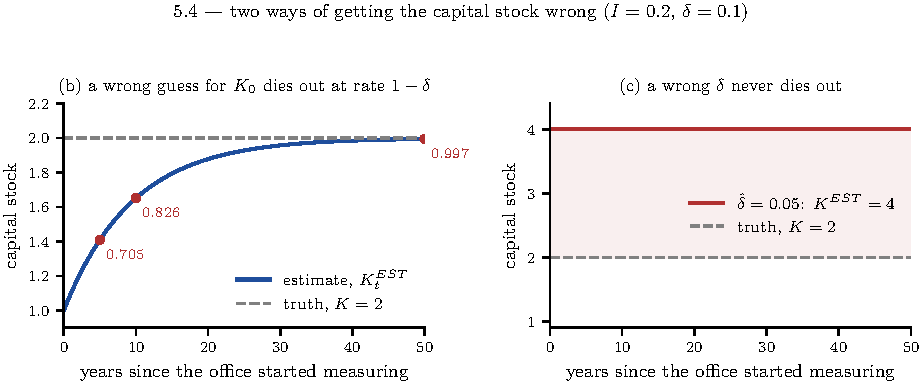
\includegraphics[width=\linewidth]{fig/fig_k5_4_capital.pdf}\\[3pt]
\captionof{figure}{Problem 5.4. A wrong initial guess (left) is forgotten at rate
$1-\delta$; a wrong depreciation rate (right) never is.}
\label{fig:cap54}
\end{center}
\end{tcolorbox}

%------- 5.5 -------
% Topic: Mismeasurement as a Source of Measured TFP
% Keywords: institutions, rent-seeking, measured TFP, factor prices, make-work policy
\begin{tcolorbox}[oddbox,title={Problem 5.5 \quad Sources of TFP}]
\begin{tcolorbox}[questionbox]
Suppose that the true production function in Gotham is
\[
Y=AK^{\alpha}L^{1-\alpha}
\tag{5.5.3}
\]
Unfortunately, crime is a huge problem in Gotham, so that for each worker doing actual work
firms need to hire $\phi$ security guards just to protect their products from being stolen.
The security guards will of course describe their activity as work even though they are not
actually producing anything. Use the notation $N$ to refer to the total labor force
(including workers and guards) and denote the number of actual production workers by
$L$.\\[3pt]
(a) Find an expression for total output as a function of $A$, $K$, $N$, $\phi$ and
$\alpha$.\\[3pt]
(b) Write down the problem of a firm that has to choose capital and labor to maximize
profits. Notice that the firm will have to pay a wage to the security guards even though
they will not produce anything.\\[3pt]
(c) If the representative firm hires all the workers and rents all the capital, what will be
the wage and the rental rate of capital? Express it as a function of $A$, $K$, $N$, $\phi$
and $\alpha$.\\[3pt]
(d) Suppose an economist studying Gotham is trying to estimate $A$ using equation (5.5.3).
The economist has accurate data on $K$, $N$ and $Y$. However, the economist doesn't really
know whether workers are involved in production or in security services: in national
statistics they all look employed. Therefore the economist will plug in the value of $N$
instead of the value of $L$ into the estimate of $A$. What will the economist's estimate of
$A$ be? How does it compare to the true value of $A$?\\[3pt]
(e) How does this relate to the findings that link GDP levels to social and political
institutions?\\[3pt]
(f) Suppose that, in an economy that didn't have the crime problem of Gotham, the government
attempted to create jobs by mandating that firms hire $\phi$ assistants for every production
worker. The job of assistants is to look at production workers all day long and not do
anything. Using the analysis above, what would be the effects of such a policy?
\end{tcolorbox}

\textbf{Solution:}
\begin{enumerate}

\item Each production worker requires $\phi$ guards, so a firm employing $L$ producers must
hire $L+\phi L$ people in total:
\[
N=(1+\phi)L
\qquad\Longrightarrow\qquad
L=\frac{N}{1+\phi} .
\]
Substituting into (5.5.3),
\[
\boxed{\;Y=AK^{\alpha}\left(\frac{N}{1+\phi}\right)^{1-\alpha}
=\underbrace{A(1+\phi)^{-(1-\alpha)}}_{\textstyle \tilde A}\,K^{\alpha}N^{1-\alpha}\;}
\tag{5.5.a}
\]
The economy behaves \emph{exactly} like one with the same total employment $N$ and a lower
Hicks-neutral productivity $\tilde A=A(1+\phi)^{-(1-\alpha)}$. That observational
equivalence is the whole exercise.

\item The firm hires $N$ people at the market wage $w$ (it must pay guards too) and rents
$K$ at $r^K$. Using (5.5.a),
\[
\max_{K,\,N}\;\;
A(1+\phi)^{-(1-\alpha)}K^{\alpha}N^{1-\alpha}-wN-r^{K}K .
\]
It is important that the firm's choice variable is $N$, not $L$: the technology $\phi$ is
imposed, so the firm cannot economise on guards, and every person on the payroll costs $w$.

\item First-order conditions:
\[
\boxed{w=(1-\alpha)\,A(1+\phi)^{-(1-\alpha)}\left(\frac{K}{N}\right)^{\alpha}},
\qquad
\boxed{r^{K}=\alpha\,A(1+\phi)^{-(1-\alpha)}\left(\frac{N}{K}\right)^{1-\alpha}} .
\]
Both are the usual Cobb-Douglas factor prices with $A$ replaced by $\tilde A$. Two remarks:
\begin{itemize}[leftmargin=1.3em,itemsep=2pt,topsep=3pt]
\item \textbf{Guards and producers earn the same wage} $w$, even though the guards produce
      nothing. In a competitive labour market a firm cannot pay two prices for the same
      labour, and it will not hire a guard unless the guard is worth $w$ to it --- which he
      is, because without him the goods are stolen. The guard's marginal product to the
      \emph{firm} is $w$; his marginal product to \emph{society} is zero.
\item Factor shares are unaffected: $wN/Y=1-\alpha$ and $r^KK/Y=\alpha$ exactly as before.
      \checkmark\ Crime is therefore invisible in the income accounts, which is why part (d)
      works.
\end{itemize}

\item The economist computes
\[
\hat A=\frac{Y}{K^{\alpha}N^{1-\alpha}}
\stackrel{\text{(5.5.a)}}{=}A(1+\phi)^{-(1-\alpha)}
\qquad\Longrightarrow\qquad
\boxed{\frac{\hat A}{A}=(1+\phi)^{-(1-\alpha)}<1} .
\]
Measured TFP is \emph{below} true TFP. With $\alpha=0.35$ and $\phi=1$ (one guard per
worker), $\hat A/A=2^{-0.65}=0.637$: Gotham looks 36\% less productive than it is.
\checkmark

\smallskip
It is worth pushing this to the long run, because that is where the number becomes
interpretable. In a Solow steady state with $Y=\tilde A K^{\alpha}N^{1-\alpha}$ and
$n=g=0$,
\[
\frac{Y}{N}\bigg|_{ss}
=\tilde A^{\frac{1}{1-\alpha}}\left(\frac{s}{\delta}\right)^{\frac{\alpha}{1-\alpha}},
\qquad
\tilde A^{\frac{1}{1-\alpha}}=A^{\frac{1}{1-\alpha}}\,\frac{1}{1+\phi},
\]
so long-run GDP per person, \emph{and the wage with it}, fall by exactly
\[
\boxed{\frac{1}{1+\phi}} ,
\]
which is one half when $\phi=1$. \checkmark\ The exponents cancel and leave something
transparent: in the long run the economy loses output in exact proportion to the fraction of
its labour force that is not producing anything. The $(1-\alpha)$ in the TFP formula is an
artefact of holding $K$ fixed; once capital adjusts, the loss is one-for-one.

\item \textbf{This is a mechanism, not just an analogy.} The cross-country evidence (\S5.5)
finds that GDP per capita correlates with rule of law, property-rights protection, control
of corruption and political stability. The natural objection is: institutions are not a
production function, so how can they show up in $A$? Gotham is the answer. Nothing about
Gotham's technology is worse --- $A$ is the same, $\alpha$ is the same, the blueprints are
the same. What differs is that weak protection of property forces the economy to spend a
fraction $\phi/(1+\phi)$ of its labour on \emph{guarding} output rather than producing it,
and the national accounts have no way to see the difference. The measured Solow residual
falls, and an economist with no other information calls it ``low TFP''.

\smallskip
Two extensions, both in the chapter:
\begin{itemize}[leftmargin=1.3em,itemsep=2pt,topsep=3pt]
\item The same argument covers any diversion of resources into activities that are privately
      valuable and socially unproductive: litigation, tax avoidance, bribery, lobbying,
      duplicated regulatory compliance. This is the theory of rent-seeking, and it predicts
      that measured TFP is a \emph{lower bound} on technological competence.
\item Hsieh and Klenow (2009) is the same idea applied to \emph{allocation} rather than
      diversion: when capital and labour sit in the wrong firms, aggregate output falls for
      given aggregate inputs, and the accounts record it as TFP. Their estimate is that
      eliminating Chinese and Indian misallocation down to US levels would raise measured TFP
      by 30--50\% and 40--60\%.
\end{itemize}

\item \textbf{A make-work mandate is arithmetically identical to crime, and it does not
create jobs.} Replace ``guards'' with ``assistants''; every equation above goes through
unchanged. Therefore:
\begin{itemize}[leftmargin=1.3em,itemsep=3pt,topsep=3pt]
\item \textbf{Employment is unchanged.} $N$ is the labour force, and it was already fully
      employed. The mandate does not create a job, it relabels $\phi/(1+\phi)$ of the
      existing ones. (Nothing in this model can generate unemployment; that machinery
      arrives in Chapter 7. But that is the point --- the policy's stated benefit does not
      exist even in principle here.)
\item \textbf{Output falls}, immediately by $(1+\phi)^{-(1-\alpha)}$ and in the long run by
      $1/(1+\phi)$.
\item \textbf{Wages fall in the same proportion}, since
      $w=(1-\alpha)\tilde A(K/N)^{\alpha}$ and $\tilde A$ has fallen. With $\phi=1$ the
      long-run wage is \emph{halved}. \checkmark\ The intended beneficiaries pay for the
      policy in full.
\item \textbf{Measured productivity falls} by $(1+\phi)^{-(1-\alpha)}$, so the statistics
      would report a technological regression that never happened.
\end{itemize}
There is one asymmetry with Gotham worth stating, and it is the policy conclusion. Gotham's
guards are a \emph{second-best response to a real problem}: given that theft exists, hiring
them is efficient, and the right intervention is to attack the crime, not the guards.
Assistants respond to no problem at all, so the policy is pure deadweight loss. The
observable consequences are identical, which is precisely why one cannot read policy
recommendations off a Solow residual.

\end{enumerate}
\end{tcolorbox}

%------- 5.9 -------
% Topic: Mismeasurement as a Source of Measured TFP
% Keywords: labour-augmenting technology, hours vs headcount, perpetual inventory, health and TFP
\begin{tcolorbox}[oddbox,title={Problem 5.9 \quad Disease and TFP}]
\begin{tcolorbox}[questionbox]
The production function in Influenzistan is
\[
Y=K^{\alpha}(AH)^{1-\alpha}
\tag{5.5.4}
\]
where $H$ is the total number of hours of work.\\[3pt]
(a) Solve equation (5.5.4) for $A$, so that you end up with an expression for $A$ in terms
of all the other variables and parameters.\\[3pt]
(b) Suppose an economist wants to measure $A$. The economist has official data from the
Influenzistan Statistics Office on: total hours worked by all workers; the total level of
investment, which has been constant for many many years; an estimate of the average rate of
depreciation of the capital stock; and GDP and its subcomponents, measured by the income
method. How can he use this data to get an estimate of $A$? Don't be vague: provide exact
formulas that describe each step precisely.\\[3pt]
(c) Suppose now that the economist has the same data as above except he doesn't know total
hours worked. Instead, the Statistics Office only keeps records on the total number of
employed workers (call this number $L$), but not on how many hours each of them works. In
order to get an estimate of $A$, the economist assumes that the average worker works $N$
hours per year, which is the number of hours worked by the average worker in neighboring
Healthistan. Write down an expression for the economist's estimate of $A$ (call this number
$\hat A$).\\[3pt]
(d) Unfortunately, the residents of Influenzistan keep getting sick, so they have to spend a
significant portion of their time recovering at home instead of working. As a result, they
each work $xN$ hours instead of $N$ hours, where $x<1$. Derive an expression for $\hat A/A$,
i.e.\ for the ratio of the economist's estimate of $A$ to its true value. Interpret your
finding.
\end{tcolorbox}

\textbf{Solution:}
\begin{enumerate}

\item Isolate the $A$ term and raise to the power $1/(1-\alpha)$:
\[
Y=K^{\alpha}A^{1-\alpha}H^{1-\alpha}
\;\Longrightarrow\;
A^{1-\alpha}=\frac{Y}{K^{\alpha}H^{1-\alpha}}
\;\Longrightarrow\;
\boxed{\;A=\frac{1}{H}\left(\frac{Y}{K^{\alpha}}\right)^{\frac{1}{1-\alpha}}\;}
\tag{5.9.a}
\]
or, written out, $A=Y^{\frac{1}{1-\alpha}}K^{-\frac{\alpha}{1-\alpha}}/H$.

\smallskip
Note the exponent on $H$: it is exactly $-1$. Because $A$ is \emph{labour-augmenting}, it
multiplies $H$ one-for-one, so any proportional error in $H$ becomes the same proportional
error in $A$. In Problem 5.4 the corresponding elasticity, of measured productivity with
respect to the capital estimate, was only $-\alpha=-0.35$; here it is $-1$. That gap is the
point of the whole problem.

\item Four steps, each tied to one of the four data items.

\begin{enumerate}[label=\textbf{Step \arabic*.},leftmargin=2.6em,itemsep=4pt,topsep=3pt]
\item \textbf{Get $\alpha$ from the income accounts.} The income-method subcomponents split
GDP into labour and capital income. Under competition the capital share equals the output
elasticity of capital, so
\[
\alpha=\frac{\text{capital income}}{Y}
=\frac{\text{operating surplus}}
       {\text{operating surplus}+\text{compensation of employees}} .
\]
This is why the exercise insists on the \emph{income} method: no other decomposition of GDP
delivers $\alpha$.

\item \textbf{Get $K$ from investment and depreciation.} Investment has been constant at $I$
``for many many years'', so the capital stock has converged to its steady state, where
$\delta K=I$ (this is exactly Problem 5.4(a)):
\[
\hat K=\frac{I}{\hat\delta} .
\]
Constancy of $I$ is what makes this legitimate --- it removes the need for a whole
investment history and for an initial condition.

\item \textbf{Read $Y$ and $H$} directly off the accounts and the hours survey.

\item \textbf{Substitute into (5.9.a):}
\[
\boxed{\;\hat A=\frac{1}{H}\left(\frac{Y}{(I/\hat\delta)^{\alpha}}\right)^{\frac{1}{1-\alpha}}\;}
\]
\end{enumerate}
\checkmark\ \texttt{problema\_5\_9()} builds an artificial economy from a known $A$, runs
these four steps, and recovers $A$ exactly.

\item Replace the unobserved $H$ by the assumed $\hat H=LN$:
\[
\boxed{\;\hat A=\frac{1}{LN}\left(\frac{Y}{(I/\hat\delta)^{\alpha}}\right)^{\frac{1}{1-\alpha}}
=\frac{Y^{\frac{1}{1-\alpha}}K^{-\frac{\alpha}{1-\alpha}}}{LN}\;}
\]

\item The true hours are $H=L\,xN$. Since $Y$, $K$ and $\alpha$ are measured correctly,
everything in the numerator of (5.9.a) is common to $\hat A$ and $A$ and cancels:
\[
\frac{\hat A}{A}
=\frac{Y^{\frac{1}{1-\alpha}}K^{-\frac{\alpha}{1-\alpha}}/(LN)}
      {Y^{\frac{1}{1-\alpha}}K^{-\frac{\alpha}{1-\alpha}}/(LxN)}
=\frac{LxN}{LN}
=\boxed{\;x\;}
\]
\checkmark

\end{enumerate}

\smallskip
\emph{Interpretation --- and this is the sharpest version of the chapter's warning.}

\begin{enumerate}[label=\textbf{\arabic*.},leftmargin=1.6em,itemsep=4pt,topsep=3pt]
\item \textbf{The bias is one-for-one and $\alpha$ does not appear.} If sickness costs 20\%
of working hours, measured TFP is 20\% too low --- not $0.8^{1-\alpha}$, not
$0.8^{\alpha}$, but exactly $0.8$. There is no dilution and no offsetting term. Compare
Problem 5.4, where doubling the capital estimate cost only 21.5\% of measured $A$: errors in
\emph{labour} input are far more damaging to a residual than errors in capital, because
labour carries the larger share and, in the labour-augmenting formulation, $A$ absorbs the
error directly.

\item \textbf{The disease is real and the productivity gap is not.} Influenzistan really is
poorer: fewer hours are worked, so $Y$ really is lower. What is spurious is the
\emph{attribution}. An economist comparing Influenzistan with Healthistan would report a
technology gap of $1-x$, when the two countries have identical technology and differ only in
how much labour they supply. The measurement error and the underlying problem point in the
same direction, which is what makes the mistake hard to catch.

\item \textbf{Consistency with Problem 5.5.} \checkmark\ The two exercises are the same trap
in different notation. In Gotham, labour input was over-counted by a factor $m=1+\phi$ and
the Hicks-neutral $\tilde A$ was biased by $m^{-(1-\alpha)}$. Here labour is over-counted by
$m=1/x$. Converting the labour-augmenting $A$ into its Hicks-neutral equivalent
$\tilde A=A^{1-\alpha}$,
\[
\frac{\hat{\tilde A}}{\tilde A}=\left(\frac{\hat A}{A}\right)^{1-\alpha}=x^{1-\alpha}
=m^{-(1-\alpha)} ,
\]
which is Gotham's formula exactly. \checkmark\ This identity is asserted in
\texttt{ch05\_numerico.py} and would abort the script if it failed. The apparent
disagreement between ``bias $=x$'' and ``bias $=m^{-(1-\alpha)}$'' is entirely about which
$A$ one is talking about.

\item \textbf{The practical moral.} This is why the development-accounting literature works
so hard on \emph{hours and human capital} rather than headcounts --- one thinks of
Hall--Jones-style adjustments for schooling, and of the Penn World Table's move to
hours-based labour input. Every quality dimension of labour that goes unmeasured --- health,
schooling, experience, hours --- is pushed wholesale into the residual with an elasticity of
one. A ``TFP difference'' between two countries is a statement about what the analyst failed
to measure at least as much as a statement about technology.
\end{enumerate}
\end{tcolorbox}

%======================================================================
\section*{Companion code}
\addcontentsline{toc}{section}{Companion code}
%======================================================================

Every numerical result above is reproduced by \texttt{Resolucao/kurlat\_ch05\_codigo/}. Each
script checks its analytical formulas against an independent numerical computation and aborts
on any mismatch.

\begin{center}
\begin{tabular}{@{}lp{10.2cm}@{}}
\toprule
\textbf{File} & \textbf{What it does} \\
\midrule
\texttt{ch05\_numerico.py} & Problem 5.1: the steady state, the two 100-year simulations, the
years to 95\%, plus a rerun under the exact (non-approximated) law of motion. Problem 5.2:
the table of $g_y$, each row cross-checked against one exact iteration of the capital
recursion, and the limit $\delta(1-\alpha)$. Problem 5.3: the steady-state decomposition.
Problem 5.4: the closed form $K\EST_t=2-(0.9)^t$ against the raw iteration, and $2^{-0.35}$.
Problem 5.5: the TFP bias and a proof that long-run output and wages fall by $1/(1+\phi)$.
Problem 5.6: the drift of $\ln(r+\delta)$ under each conjecture. Problems 5.7 and 5.8: the
three GDP methods, asserted equal; the factor shares; the interest rate; the growth
accounting; and a grid search confirming that $s_{gr}=\alpha$. Problem 5.9: an artificial
economy in which the four-step estimator recovers $A$ exactly, the bias is exactly $x$, and
the Gotham formula is recovered after converting to Hicks-neutral units. \\
\texttt{ch05\_figuras.py} & The three figures. \\
\texttt{estilo\_mpl.py} & \texttt{pgf} backend, so figure text is typeset by \texttt{pdflatex}
with \texttt{lmodern} and \texttt{cmap} and the PDF stays fully copyable. \\
\bottomrule
\end{tabular}
\end{center}

\end{document}
